% \documentclass[tikz,convert={density=300,size=1080x800,outext=.png}]{standalone}
\documentclass[tikz,convert=false]{standalone}
\usetikzlibrary{mindmap,trees,graphs,calc,shapes.geometric,positioning}
\usepackage{amsmath,amssymb,amsthm,mathrsfs,mathtools,xcolor}

\newcommand{\R}{\mathbb{R}}
\newcommand{\Norm}[1]{\left|\left|  #1   \right|\right|}
\newcommand{\E}{\mathbb{E}}
\newcommand{\FoxH}[5]{H_{#2}^{#1}\left(#3\:\middle\vert\: \begin{subarray}{l}#4\\[0.4em] #5\end{subarray}\right)}
\newcommand{\Res}{\mathop{\text{Res}}}

\begin{document}
  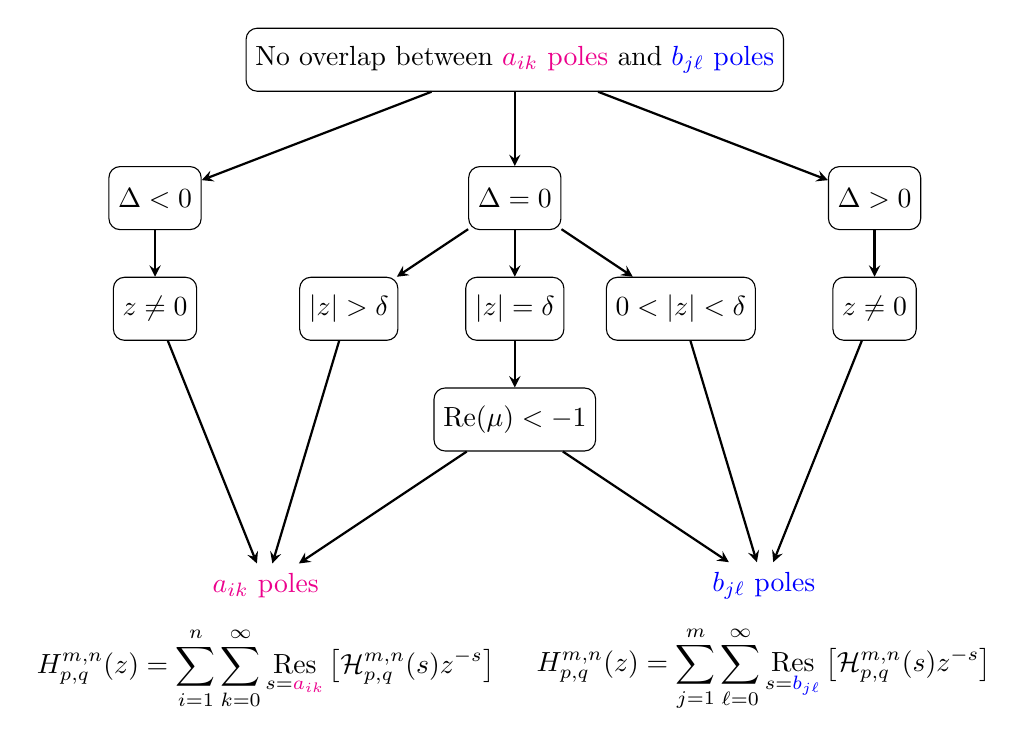
\begin{tikzpicture}[scale=1, transform shape, node distance = 4em, auto]
    \tikzset{>=latex}
    % Draw a rectangle node
    \tikzstyle{poles}  = [rectangle, rounded corners, minimum width  = 3cm, minimum height = 0.8cm, text centered, draw = black, fill = white]
    \tikzstyle{others} = [rectangle, rounded corners, minimum width  = 1cm, minimum height = 0.8cm, text centered, draw = black, fill = white]
    \tikzstyle{Res}    = [minimum width  = 10cm, minimum height = 0.8cm, text centered, fill = white]
    \tikzstyle{arrow}  = [thick,->,  >= stealth]

    \node[poles] (poles) at (0,0) {No overlap between \textcolor{magenta}{$a_{ik}$ poles} and \textcolor{blue}{$b_{j\ell}$ poles}};
    % \node[others, below of = poles] (Nonzero) {$z\ne 0$};
    \node[others, below of = poles, yshift = -1em] (D0) {$\Delta = 0$};
    \node[others, xshift = -9em, left of  = D0] (DN) {$\Delta < 0$};
    \node[others, xshift = +9em, right of = D0] (DP) {$\Delta > 0$};
    \node[others, below of = D0] (D00) {$|z| = \delta$};
    \node[others, xshift = -2em, left of  = D00] (D0P) {$|z|>\delta$};
    \node[others, xshift = +2em, right of = D00] (D0N) {$0<|z|<\delta$};
    \node[others, below of = D00] (D000) {$\text{Re}(\mu)<-1$};

    \node[others, below of = DN] (DN0) {$z\ne 0$};
    \node[others, below of = DP] (DP0) {$z\ne 0$};

    \node[below of = D000, xshift = +9em, yshift = -2em, blue] (b) {$b_{j\ell}$ poles};
    \node[below of = D000, xshift = -9em, yshift = -2em, magenta] (a) {$a_{ik}$ poles};

    \node[below of = b, yshift = +1em] (bf) {$ \displaystyle H_{p,q}^{m,n}(z) = \sum_{j=1}^{m} \sum_{\ell=0}^{\infty} \Res_{s = \textcolor{blue}{b_{j\ell}}} \left[\mathcal{H}_{p,q}^{m,n}(s) z^{-s}\right]$};
    \node[below of = a, yshift = +1em] (af) {$ \displaystyle H_{p,q}^{m,n}(z) = \sum_{i=1}^{n} \sum_{k=0}^{\infty}    \Res_{s = \textcolor{magenta}{a_{ik}}} \left[\mathcal{H}_{p,q}^{m,n}(s) z^{-s}\right]$};

    \draw[arrow] (poles) -- (D0);
    \draw[arrow] (poles) -- (DN);
    \draw[arrow] (poles) -- (DP);
    \draw[arrow] (D0) -- (D00);
    \draw[arrow] (D0) -- (D0P);
    \draw[arrow] (D0) -- (D0N);
    \draw[arrow] (D00) -- (D000);

    \draw[arrow] (DN) -- (DN0);
    \draw[arrow] (DP) -- (DP0);

    \draw[arrow] (DN0) -- (a);
    \draw[arrow] (DP0) -- (b);

    \draw[arrow] (D0N)  -- (b);
    \draw[arrow] (D0P)  -- (a);
    \draw[arrow] (D000) -- (a);
    \draw[arrow] (D000) -- (b);
  \end{tikzpicture}
\end{document}
